\chapter{Tracking, Spin, and Transfer Matrix Calculation Methods}
\label{c:methods}

\index{element!class}\index{tracking_method}
\index{mat6_calc_method}\index{spin_tracking_method}
\bmad allows for a number of methods that can be use to ``track'' a particle
through a lattice element. Here ``track'' can mean one of three things:
\begin{example}
  1) Calculate a particle's phase space coordinates at the exit 
     end of the element given the coordinates at the entrance end.
  2) Calculate the linear transfer map (Jacobian) through an element
     about a given reference orbit.
  3) Calculate the a particle's spin orientation at the exit end 
     of the element given the coordinates at the beginning.
\end{example}
The different tracking methods that are available have different
advantages and disadvantages in terms of speed, symplecticity, etc.
What tracking method is used, is selected on an element--by--element
basis using the attributes:
\begin{example}
  tracking_method      = <Switch>   ! phase space tracking method.
  mat6_calc_method     = <Switch>   ! 6x6 transfer matrix calculation.
  spin_tracking_method = <Switch>   ! Spin tracking method.
\end{example}
Example:
\begin{example}
  q2: quadrupole, tracking_method = boris
  q2[tracking_method] = boris
  quadrupole[tracking_method] = boris
\end{example}
The first two lines of this example have exactly the same effect in
terms of setting the \vn{tracking_method}. The third line shows how to
set the \vn{tracking_method} for an entire class of elements.

These switches are discussed in more detail in the following sections.

%----------------------------------------------------------------------------
\section{Particle Tracking Methods}
\label{s:tkm}
\index{tracking methods|hyperbf}

The \vn{tracking_method} attribute of an element sets the algorithm
that is used for single particle tracking through that element.
Table~\ref{t:track.methods} gives which methods are available for each
type of element.

A note on terminology: Adaptive step size control used with the
\vn{Runge_Kutta} integrator means that instead of taking fixed step
sizes the integrator chooses the proper step size so that the error in
the tracking is below the maximum allowable error set by \vn{rel_tol}
and \vn{abs_tol} tolerances. The advantage of step size control is
that the integrator uses a smaller step size when needed (the fields
are rapidly varying), but makes larger steps when it can. The
disadvantage is that a step is more computationally intensive since
the error in a step is estimated by repeating a step using two mini
steps. If the fields are rather uniform and you know what a good step
size is you can save time by using a fixed step size.

\begin{figure}[tb]
  \centering
  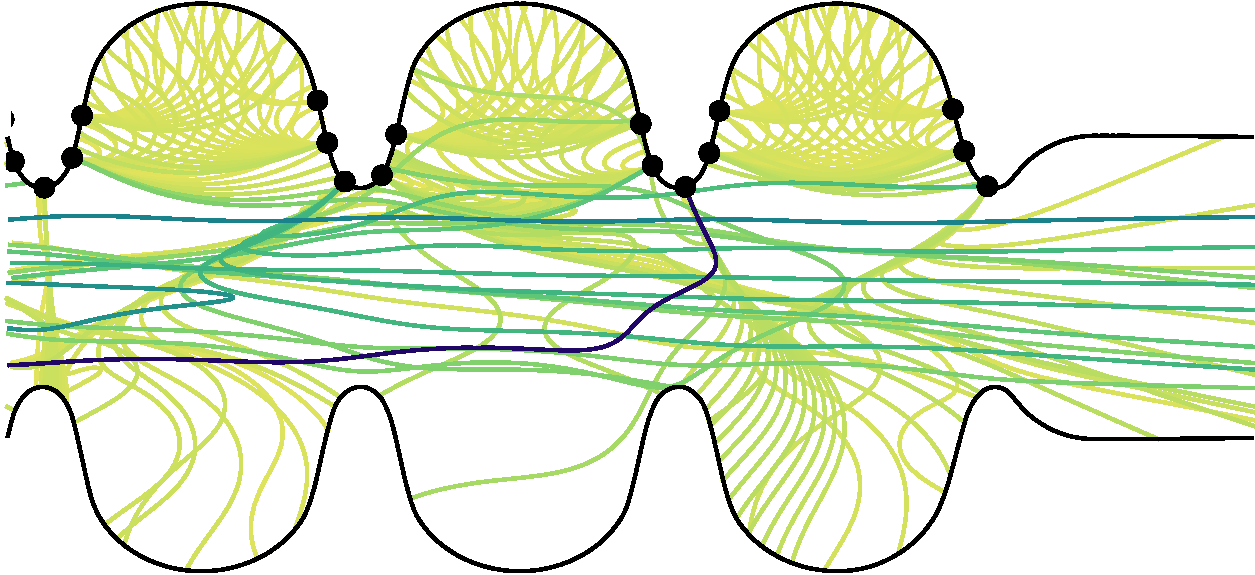
\includegraphics[width=4in]{dark-current.pdf}
  \caption[Dark current tracking.]{
Dark current tracking. Example of where a time based tracker (\vn{time_runge_kutta}) is
useful for simulating particles that can reverse their longitudinal velocity. Here the
tracks drawn are from a simulation of ``dark current'' electrons generated at the
walls of an RF cavity due to the large electromagnetic fields.
}
  \label{f:dark.current}
\end{figure}

\begin{description}

\index{boris!tracking_method}
\item[\vn{Boris}]
Second order Boris Integration\cite{b:boris}. Like \vn{Runge_Kutta},
\vn{Boris} does tracking by integrating the equation of
motion. \vn{Boris} handles both electric and magnetic fields and does
not assume that the particle is ultra--relativistic. \vn{Boris} preserves
conserved quantities more accurately than \vn{Runge_Kutta}.

\index{bmad_standard!tracking_method}
\item[\vn{Bmad_Standard}]
Uses formulas for tracking. The formulas generally use the paraxial
approximation.  The emphasis here is on speed. Note: If an element has
non-zero multipole values, \vn{Bmad_Standard} tracking will generally
put half the multipole kick at the beginning of the element and half
at the end. This is generally a good approximation but in it can
result in differences between this and tracking methods like
\vn{Symp_Lie_PTC} which model multipoles as as distributed evenly
throughout an element.

\index{custom!tracking_method}
\item[\vn{Custom}]
This method will call a routine \vn{track1_custom} which must be
supplied by the programmer implementing the custom tracking. The
default \vn{track1_custom} supplied with the \bmad release will print
an error message and stop the program if it is called which probably
indicates a program linking problem. See \vn{s:custom.ele} for more details.

\index{linear!tracking_method}
\item[\vn{Linear}]
Linear just uses the 0th order vector with the 1st order 6x6 transfer
matrix for an element. Very simple.  Depending upon how the transfer
matrix was generated this may or may not be symplectic.

\index{MAD!tracking_method}
\item[\vn{MAD}]
This uses the MAD 2nd order transfer map. This method is not able to
handle element misalignments or kicks, and becomes inaccurate as the
particle energy deviates from the reference energy. MAD tracking is
generally only used for testing purposes. Note: Thanks to CERN and
Frank Schmidt for permission to use the MAD tracking code within
\bmad.

\index{runge_kutta!tracking_method}
\item[\vn{runge_kutta}]
This uses a 4\Th order Runge Kutta integration algorithm with adaptive
step size control.  This is essentially the \vn{ODEINT} subroutine
from Numerical Recipes\cite{b:nr}. This may be slow but it should be
accurate. This method is non-symplectic. \vn{Warning:} When using
\vn{custom} fields, if the fields do not obey Maxwell's equation,
there is the possibility of the \vn{runge_kutta} tracking halting mid
way through an element. See section~\sref{s:integ} for more details.

\index{symp_lie_Bmad!tracking_method}
\item[\vn{Symp_Lie_Bmad}]
Symplectic tracking using a Hamiltonian with Lie operation techniques.
This is similar to \vn{Symp_Lie_PTC} (see below) except this uses a
\bmad routine. By bypassing some of the generality inherent in PTC
(\sref{s:ptc.intro}), \vn{Symp_Lie_Bmad} achieves about a factor of 10
improvement in speed over \vn{Symp_Lie_PTC}.

\index{symp_lie_ptc!tracking_method}
\item[\vn{Symp_Lie_PTC}]
Symplectic tracking using a Hamiltonian with Lie operator techniques.
This uses \'Etienne Forest's PTC (\sref{s:ptc.intro}) software for the
calculation. This method is symplectic but can be slow.

\index{symp_map!tracking_method}
\item[\vn{Symp_Map}]
This uses a partially inverted, implicit Taylor map. The calculation
uses \'Etienne Forest's PTC software (\sref{s:ptc.intro}).  Since the
map is implicit, a Newton search method must be used. This will slow
things down from the Taylor method but this is guaranteed
symplectic. Note: Due to memory limitations in PTC, the number of
elements using symp_map is limited to be of order 50.

\index{taylor!tracking_method}
\item[\vn{Taylor}]
This uses a Taylor map generated from the PTC (\sref{s:ptc.intro})
package. Generating the map may take time but once you have it it
should be very fast. One possible problem with using a Taylor map is
that you have to worry about the accuracy if you do tracking at points
that are far from the expansion point about which the map was
made. This method is non-symplectic away from the expansion
point. Whether the Taylor map is generated taking into account the
offset an element has is governed by the \vn{taylor_map_includes_offsets}
attribute (\sref{s:mapoff}).  

The order of a Taylor map is set by the \vn{parameter[taylor_order]}
parameter (\sref{s:param}).

Note: Taylor maps for \vn{match} elements are limited to first order.

\index{time_runge_kutta!tracking_method}
\item[\vn{Time_Runge_Kutta}]
This method uses time as the independent variable instead of the longitudinal $z$
position. The advantage of this method is that it can handle particles which reverse
direction longitudinally.  One use for this method is ``dark current'' tracking where, as
illustrated in \fig{f:dark.current}, low energy particles generated at the vacuum chamber
walls can be found traveling in all directions. Notice that \vn{time_runge_kutta} is
different from using \vn{absolute time tracking} as explained in \sref{s:rf.time}.

\end{description}

%----------------------------------------------------------------------------

\index{ab_multipole}\index{beambeam}\index{bend_sol_quad}\index{custom}
\index{drift}\index{ecollimator}\index{elseparator}\index{hkicker}
\index{instrument}\index{kicker}\index{lcavity}\index{marker}
\index{match}\index{monitor}\index{multipole}\index{octupole}
\index{patch}\index{quadrupole}\index{rbend}\index{rcollimator}
\index{rfcavity}\index{sbend}\index{sextupole}\index{solenoid}
\index{sol_quad}\index{taylor}\index{vkicker}\index{wiggler}\index{capillary}
\index{element!table of class types}
\begin{table}[pht]
\centering {
\begin{tabular}{lcccccccccccc} \toprule
\rule{0pt}{80pt} 
{\em Element Class} &
\begin{sideways}\vn{Bmad_Standard}\end{sideways} &
\begin{sideways}\vn{Boris}\end{sideways} &
\begin{sideways}\vn{Custom}\end{sideways} &
\begin{sideways}\vn{Linear}\end{sideways} &
\begin{sideways}\vn{MAD}\end{sideways} &
\begin{sideways}\vn{Runge_Kutta}\end{sideways} &
\begin{sideways}\vn{Symp_Lie_Bmad}\end{sideways} &
\begin{sideways}\vn{Symp_Lie_PTC}\end{sideways} &
\begin{sideways}\vn{Symp_Map}\end{sideways} &
\begin{sideways}\vn{Taylor}\end{sideways} &
\begin{sideways}\vn{Time_Runge_Kutta}\end{sideways} &
\\ \midrule
%                               BS   B   C   L   M   RK    SLB   SLP   SM     T   TRK
  \vn{ab_multipole}            & D &   & X & X &   &     &     &  X  &  X  &  X  &    \\  
  \vn{beambeam}                & D &   & X & X &   &     &     &     &     &     &    \\  
  \vn{bend_sol_quad}           &   &   & X &   &   &     &  D  &     &     &     &    \\  
  \vn{capillary}               & D &   & X &   &   &     &     &     &     &     &    \\  
  \vn{crystal}                 & D &   & X &   &   &     &     &     &     &     &    \\  
  \vn{custom}                  &   & X & D & X &   &  X  &     &     &     &     & X  \\  
  \vn{drift}                   & D & X & X & X & X &  X  &     &  X  &  X  &  X  & X  \\  
  \vn{e_gun}                   &   &   & X &   &   &     &     &     &     &     & D  \\  
  \vn{ecollimator}             & D & X & X & X &   &  X  &     &  X  &  X  &  X  & X  \\  
  \vn{elseparator}             & D & X & X & X & X &  X  &     &  X  &  X  &  X  & X  \\  
  \vn{em_field}                &   & X & X &   &   &  D  &     &     &     &     & X  \\  
  \vn{floor_shift}             & D &   & X &   &   &     &     &     &     &     &    \\  
  \vn{hkicker}                 & D & X & X & X &   &  X  &     &  X  &  X  &  X  & X  \\  
  \vn{instrument}              & D & X & X & X &   &  X  &     &  X  &  X  &  X  & X  \\  
  \vn{kicker}                  & D & X & X & X &   &  X  &     &  X  &  X  &  X  & X  \\  
  \vn{lcavity}                 & D & X & X & X &   &  X  &     &  X  &  X  &  X  & X  \\  
  \vn{marker}                  & D &   & X & X &   &     &     &  X  &  X  &  X  &    \\  
  \vn{match}                   & D &   & X &   &   &     &     &     &     &  *  &    \\ 
  \vn{monitor}                 & D & X & X & X &   &  X  &     &  X  &  X  &  X  & X  \\  
  \vn{mirror}                  & D &   & X &   &   &     &     &     &     &     &    \\  
  \vn{multipole}               & D &   & X & X &   &     &     &  X  &  X  &  X  &    \\  
  \vn{multilayer}              & D &   & X &   &   &     &     &     &     &     &    \\  
  \vn{octupole}                & D & X & X & X &   &  X  &     &  X  &  X  &  X  & X  \\ 
  \vn{patch}                   & D &   & X &   &   &  X  &     &  X  &     &  X  &    \\ 
  \vn{quadrupole}              & D & X & X & X & X &  X  &  X  &  X  &  X  &  X  & X  \\ 
  \vn{rbend}                   & D &   & X & X & X &     &     &  X  &  X  &  X  &    \\ 
  \vn{rcollimator}             & D & X & X & X &   &  X  &     &  X  &  X  &  X  & X  \\ 
  \vn{rfcavity}                & D & X & X & X & X &  X  &     &  X  &  X  &  X  & X  \\ 
  \vn{sad_mult}                & D &   & X & X &   &     &     &  X  &  X  &  X  &    \\
  \vn{sample}                  & D &   & X &   &   &     &     &     &     &     &    \\
  \vn{sbend}                   & D &   & X & X & X &  X  &     &  X  &  X  &  X  & X  \\ 
  \vn{sextupole}               & D & X & X & X & X &  X  &     &  X  &  X  &  X  & X  \\ 
  \vn{solenoid}                & D & X & X & X & X &  X  &  X  &  X  &  X  &  X  & X  \\ 
  \vn{sol_quad}                & D & X & X & X &   &  X  &  X  &  X  &  X  &  X  & X  \\ 
  \vn{taylor}                  & X &   & X & X &   &     &     &     &     &  D  &    \\ 
  \vn{vkicker}                 & D & X & X & X &   &  X  &     &  X  &  X  &  X  & X  \\ 
  \vn{wiggler} (map type)      &   & X & X & X &   &  X  &  X  &  X  &  X  &  X  & X  \\
  \vn{wiggler} (periodic type) & D & X & X & X &   &X$^a$&X$^a$&X$^a$&X$^a$&X$^a$&    \\ \bottomrule
   \multicolumn{12}{l}{$^a$See \sref{s:wiggler.periodic} for more details} \\
\end{tabular}
} 
\caption[Table of available {\bf tracking_method}\ switches for a
given element class.]{Table of available {\bf tracking_method}\
switches for a given element class. ``D'' denotes the default
method. ``X'' denotes an available method. ``*'' denotes that the
Taylor map will only be first order. 
}

\label{t:track.methods}
\end{table}

\vfill \break

%----------------------------------------------------------------------------
\section{Linear Transfer Map Methods}
\label{s:xfer}
\index{mat6_calc_method|hyperbf}

The \vn{mat6_calc_method} attribute sets how the 6x6 Jacobian transfer
matrix for a given element is computed.  Table~\ref{t:mat6.methods}
gives which methods are available for each type of element.

\index{sympliectify}
\index{taylor_map_includes_offsets}
In addition to the \vn{mat6_calc_method} switch, 
two element attributes that can affect the way the transfer matrix is
calculated are \vn{symplectify} and \vn{taylor_map_includes_offsets}. These are
discussed in sections \sref{s:symp} and \sref{s:mapoff} respectively.

For methods that do not necessarily produce a symplectic matrix the
\vn{symplectify} attribute of an element can be set to \vn{True} to
solve the problem. See \sref{s:symp.method}. 

Symplectic integration is like ordinary integration of a function f(x)
but what is integrated here is a Taylor map. Truncating the map to
0\Th order gives the particle trajectory and truncating to 1\St\
order gives the transfer matrix (Jacobian).  The order at which a
Taylor series is truncated at is set by \vn{taylor_order} (see
\sref{s:param}. Like ordinary integration there are various
formulas that one can use to do symplectic integration. In \bmad (or
more precisely in PTC (\sref{s:ptc.intro})) you can use one of 3 methods. This is
set by \vn{integrator_order}.  \vn{integrator_order} = n where $n$ is
allowed by PTC to be 2, 4, or 6. With an integration order of $n$ the
error in an integration step scales as $dz^n$ where $dz$ is step
size. The step size $dz$ is set by the length of the element and the
value of \vn{ds_step}. Remember, as in ordinary integration, higher
integration order does not necessarily imply higher accuracy.

\begin{description}

\index{bmad_standard!mat6_calc_method}
\item[\vn{Bmad_Standard}]
Uses formulas for the calculation. The formulas generally use the
paraxial approximation. The emphasis here is on speed.

\index{custom!mat6_calc_method}
\item[\vn{Custom}]
This method will call a routine \vn{make_mat6_custom} which must be
supplied by the programmer implementing the custom transfer matrix
calculation. The default \vn{make_mat6_custom} supplied with the
\bmad release will print an error message and stop the program if it
is called which probably indicates a program linking problem.
See \vn{s:custom.ele} for more details.

\index{MAD!mat6_calc_method}
\item[\vn{MAD}]
This uses the MAD 2nd transfer map. This method is not able to
handle element misalignments or kicks, and becomes inaccurate as the
particle energy deviates from the reference energy. MAD tracking is
generally only used for testing purposes. Thanks must be given
to CERN and Frank Schmidt for permission to use the MAD tracking code
within \bmad.

\index{static!mat6_calc_method}
\item[\vn{Static}]
This prevents the transfer matrix from being recomputed.
Using \vn{Static} in the input file is generally not a good idea since
it prevents the matrix from being computed in the first place.
Typically \vn{Static} is used internally in a program to prevent recomputation.

\index{symp_lie_bmad!mat6_calc_method}
\item[\vn{Symp_Lie_Bmad}]
A symplectic calculation using a Hamiltonian with Lie operator
techniques.  This is similar to \vn{Symp_Lie_PTC} (see below) except
this uses a \bmad routine. By bypassing some of the generality
inherent in PTC, \vn{Symp_Lie_Bmad} achieves about a factor
of 10 improvement in speed over \vn{Symp_Lie_PTC}. However,
\vn{Symp_Lie_Bmad} cannot generate maps above first order.

\index{symp_lie_ptc!mat6_calc_method}
\item[\vn{Symp_Lie_PTC}]
Symplectic integration using a Hamiltonian and Lie operators.
This uses the PTC (\sref{s:ptc.intro}) software for the calculation.
This method is symplectic but can be slow.

\index{symp_map!tracking_method}
\item[\vn{Symp_Map}]
This uses a partially inverted, implicit Taylor map. The calculation
uses \'Etienne Forest's PTC software (\sref{s:ptc.intro}).  Since the map is implicit, a Newton
search method must be used. This will slow things down from the Taylor
method but this is guaranteed symplectic. Note: Due to memory limitations
in PTC, the number of elements using symp_map is limited to be of order 50.

\index{taylor!mat6_calc_method}
\item[\vn{Taylor}]
This uses a Taylor map generated from \'Etienne's PTC
package. Generating the map may take time but once you have it it
should be very fast. One possible problem with using a Taylor map is
that you have to worry about the accuracy if you do a calculation at
points that are far from the expansion point about which the map was
made. This method is non-symplectic away from the expansion
point. Whether the Taylor map is generated taking into account the
offset an element has is governed by the \vn{taylor_map_includes_offsets}
attribute (\sref{s:mapoff}). \vn{bmad_standard} and \vn{taylor}
tracking methods are identical. Note: Taylor maps for \vn{match}, and
\vn{patch} elements are limited to first order.

The order of a Taylor map is set by the \vn{parameter[taylor_order]}
parameter (\sref{s:param}).

\index{tracking!mat6_calc_method}
\item[\vn{Tracking}]
This uses the tracking method set by \vn{tracking_method} to track 6
particles around the central orbit. This method is susceptible to inaccuracies
caused by nonlinearities. Furthermore this method
is almost surely slow. While non--symplectic, the advantage of this method
is that it is directly related to any tracking results.

\end{description}

\index{ab_multipole}\index{beambeam}\index{bend_sol_quad}\index{custom}
\index{drift}\index{ecollimator}\index{elseparator}\index{hkicker}
\index{instrument}\index{kicker}\index{lcavity}\index{marker}
\index{match}\index{monitor}\index{multipole}\index{octupole}
\index{patch}\index{quadrupole}\index{rbend}\index{rcollimator}
\index{rfcavity}\index{sbend}\index{sextupole}\index{solenoid}
\index{sol_quad}\index{taylor}\index{vkicker}\index{wiggler}
\index{crystal}\index{capillary}
\begin{table}[pth]
\centering {
\begin{tabular}{lcccccccc} \toprule
\rule{0pt}{80pt} &
\begin{sideways}\vn{Bmad_Standard}\end{sideways} &
\begin{sideways}\vn{Custom}\end{sideways} &
\begin{sideways}\vn{MAD}\end{sideways} &
\begin{sideways}\vn{Static}\end{sideways} &
\begin{sideways}\vn{Symp_Lie_Bmad}\end{sideways} &
\begin{sideways}\vn{Symp_Lie_PTC}\end{sideways} &
\begin{sideways}\vn{Taylor}\end{sideways} &
\begin{sideways}\vn{Tracking}\end{sideways}
\\ \midrule
%                               BS   C   M  Stat SLB   SLP   Tlr  Trk 
  \vn{ab_multipole}            & D & X &   & X &     &  X  &  X  & X \\  
  \vn{beambeam}                & D & X &   & X &     &     &     & X \\  
  \vn{bend_sol_quad}           &   & X &   & X &  D  &     &     & X \\  
  \vn{capillary}               & D & X &   & X &     &     &     & X \\  
  \vn{crystal}                 & D & X &   & X &     &     &     & X \\  
  \vn{custom}                  &   & D &   & X &     &     &     & X \\  
  \vn{drift}                   & D & X & X & X &     &  X  &  X  & X \\  
  \vn{e_gun}                   &   & X &   & X &     &     &     & D \\  
  \vn{ecollimator}             & D & X &   & X &     &  X  &  X  & X \\  
  \vn{elseparator}             & D & X & X & X &     &  X  &  X  & X \\  
  \vn{em_field}                &   & X &   & X &     &     &     & D \\  
  \vn{floor_shift}             & D & X &   & X &     &     &     & X \\  
  \vn{hkicker}                 & D & X &   & X &     &  X  &  X  & X \\  
  \vn{instrument}              & D & X &   & X &     &  X  &  X  & X \\  
  \vn{kicker}                  & D & X &   & X &     &  X  &  X  & X \\  
  \vn{lcavity}                 & D & X &   & X &     &  X  &  X  & X \\  
  \vn{marker}                  & D & X &   & X &     &  X  &  X  & X \\  
  \vn{match}                   & D & X &   & X &     &     &     & X \\  
  \vn{mirror}                  & D & X &   & X &     &     &     & X \\  
  \vn{monitor}                 & D & X &   & X &     &  X  &  X  & X \\  
  \vn{multipole}               & D & X &   & X &     &  X  &  X  & X \\  
  \vn{multilayer_mirror}       & D & X &   & X &     &     &     & X \\  
  \vn{octupole}                & D & X &   & X &     &  X  &  X  & X \\ 
  \vn{patch}                   & D & X &   & X &     &  X  &  X  & X \\ 
  \vn{quadrupole}              & D & X & X & X &  X  &  X  &  X  & X \\ 
  \vn{rbend}                   & D & X & X & X &     &  X  &  X  & X \\ 
  \vn{rcollimator}             & D & X &   & X &     &  X  &  X  & X \\ 
  \vn{rfcavity}                & D & X & X & X &     &  X  &  X  & X \\ 
  \vn{sad_mult}                & D & X &   & X &     &  X  &  X  & X \\ 
  \vn{sample}                  & D & X &   & X &     &     &     & X \\ 
  \vn{sbend}                   & D & X & X & X &     &  X  &  X  & X \\ 
  \vn{sextupole}               & D & X & X & X &     &  X  &  X  & X \\ 
  \vn{solenoid}                & D & X & X & X &  X  &  X  &  X  & X \\ 
  \vn{sol_quad}                & D & X & X & X &  X  &  X  &  X  & X \\ 
  \vn{taylor}                  & X & X &   & X &     &     &  D  &   \\ 
  \vn{vkicker}                 & D & X &   & X &     &  X  &  X  & X \\ 
  \vn{wiggler}                 & D & X &   & X &X$^a$&X$^a$&X$^a$& X \\ \bottomrule
  \multicolumn{9}{l}{$^a$See \sref{s:wiggler.periodic} for more details} \\
\end{tabular}
}
\caption[Table of available \vn{mat6_calc_method}\ switches for a
given element class.]{Table of available \vn{mat6_calc_method}\
switches for a given element class. ``D'' denotes the default
method. ``X'' denotes an available method.}

\label{t:mat6.methods}
\end{table}

\vfill \break

%----------------------------------------------------------------------------
\section{Spin Tracking Methods}
\label{s:spin.methods}
\index{spin tracking!methods}
\index{spin_tracking_method}

The \vn{spin_tracking_method} attribute of an elements sets the
algorithm that is used for tracking a particle's spin
(\sref{s:spin.dyn}) through that element. Table~\ref{t:spin.methods}
gives which methods are available for each type of element.

Since speed may be an issue, \bmad has an global parameter called
\vn{spin_tracking_on} which is part of the \vn{bmad_com} instance
(\sref{s:bmad.params}) that determines whether spin is tracked or not.

\index{spin_fringe_on}
The \vn{spin_fringe_on} element attribute (\sref{s:fringe.at}) can be used to toggle
whether the fringe fields of an element affect the spin.

\etcetc

Possible \vn{spin_tracking_method} settings are:
\begin{description}

\index{bmad_standard!spin_tracking_method}
\item[\vn{Bmad_Standard}] \Newline
Uses thick element formulas for the calculation. The emphasis here is on speed at the
potential cost of accuracy. 

\index{custom!spin_tracking_method}
\item[\vn{Custom}] \Newline
This method will call a routine \vn{track1_spin_custom} which must be
supplied by the programmer implementing the custom spin tracking
calculation. See \vn{s:custom.ele} for more details.

\index{tracking!mat6_calc_method}
\item[\vn{Tracking}] \Newline
How spin is tracked here will depend also on the setting of \vn{tracking_method}. If
\vn{tracking_method} is set to \vn{boris}, \vn{runge_kutta}, \vn{time_runge_kutta}, or
\vn{symp_lie_ptc}, the spin will be tracked along with the phase space particle
coordinates using the local fields. For all other \vn{tracking_method}s, the spin will be
tracked using the \vn{bmad_standard} spin tracking method.

\index{symp_lie_ptc!spin_tracking_method}
\item[\vn{Symp_Lie_PTC}] \Newline
Symplectic integration using a Hamiltonian and Lie operators.  This uses \'Etienne's PTC
software for the calculation.  This method is symplectic but can be slow.

\end{description}

Example:
\begin{example}
  q: quadrupole, spin_tracking_method = symp_lie_ptc
\end{example}


\index{ab_multipole}\index{beambeam}\index{bend_sol_quad}\index{custom}
\index{drift}\index{ecollimator}\index{elseparator}\index{hkicker}
\index{instrument}\index{kicker}\index{lcavity}\index{marker}
\index{match}\index{monitor}\index{multipole}\index{octupole}
\index{patch}\index{quadrupole}\index{rbend}\index{rcollimator}
\index{rfcavity}\index{sbend}\index{sextupole}\index{solenoid}
\index{sol_quad}\index{taylor}\index{vkicker}\index{wiggler}
\index{crystal}\index{capillary}
\begin{table}[pth]
\centering {
\begin{tabular}{lcccc} \toprule
\rule{0pt}{80pt} &
\begin{sideways}\vn{Bmad_Standard}\end{sideways} &
\begin{sideways}\vn{Custom}\end{sideways} &
\begin{sideways}\vn{Symp_Lie_PTC}\end{sideways} &
\begin{sideways}\vn{Tracking}\end{sideways}
\\ \midrule
%                               BS   C  SLP Trk 
  \vn{ab_multipole}            & X & X &   & D \\  
  \vn{beambeam}                &   & X &   &   \\  
  \vn{bend_sol_quad}           & X & X & X & D \\  
  \vn{capillary}               &   &   &   &   \\  
  \vn{crystal}                 &   &   &   &   \\  
  \vn{custom}                  &   & D &   & X \\  
  \vn{drift}                   & X & X & X & D \\  
  \vn{e_gun}                   &   & X &   & D \\  
  \vn{ecollimator}             & X & X & X & D \\  
  \vn{elseparator}             & X & X & X & D \\  
  \vn{em_field}                &   & X &   & D \\  
  \vn{hkicker}                 & X & X & X & D \\  
  \vn{instrument}              & X & X & X & D \\  
  \vn{kicker}                  & X & X & X & D \\  
  \vn{lcavity}                 & X & X & X & D \\  
  \vn{marker}                  & X & X & X & D \\  
  \vn{match}                   &   & X &   &   \\  
  \vn{mirror}                  &   &   &   &   \\  
  \vn{monitor}                 & X & X & X & D \\  
  \vn{multipole}               & X & X & X & D \\  
  \vn{multilayer}              &   &   &   &   \\  
  \vn{octupole}                & X & X & X & D \\ 
  \vn{patch}                   &   & X & X &   \\ 
  \vn{quadrupole}              & X & X & X & D \\ 
  \vn{rbend}                   & X & X & X & D \\ 
  \vn{rcollimator}             & X & X & X & D \\ 
  \vn{rfcavity}                & X & X & X & D \\ 
  \vn{sad_mult}                &   & X &   &   \\  
  \vn{sample}                  &   &   &   &   \\  
  \vn{sbend}                   & X & X & X & D \\ 
  \vn{sextupole}               & X & X & X & D \\ 
  \vn{solenoid}                & X & X & X & D \\ 
  \vn{sol_quad}                & X & X & X & D \\ 
  \vn{taylor}                  &   &   &   &   \\ 
  \vn{vkicker}                 & X & X & X & D \\ 
  \vn{wiggler}                 & X & X & X & D \\ \bottomrule
\end{tabular}
}

\caption[Table of available \vn{spin_tracking_method}\ switches for a
given element class.]{Table of available \vn{spin_tracking_method}\
switches for a given element class. ``D'' denotes the default
method. ``X'' denotes an available method.}

\label{t:spin.methods}
\end{table}

\vfill \break

%-----------------------------------------------------------------
\section{Integration Methods}
\label{s:integ}
\index{integration methods}

\index{symp_lie_bmad!and Taylor maps}
\index{symp_lie_ptc!and Taylor maps}
\index{taylor!and Taylor maps}
``Integration methods'' are tracking methods that involve integrating
through an element's magnetic and electric fields.  Integration
methods are split into two classes: Those that involve Taylor maps and
those that simply track a particle's position.  The Taylor map methods
are
\begin{example}
  symp_lie_bmad
  symp_lie_ptc    ! Uses PTC
  taylor          ! Uses PTC
\end{example}
See section \sref{s:taylor.phys} for more information on Taylor maps
and symplectic integration. The latter two methods involve using the
PTC library (\sref{s:ptc.intro}).

The methods that do not involve Taylor maps are
\index{boris!and Taylor maps}
\index{runge_kutta!and Taylor maps}
\begin{example}
  boris
  runge_kutta
  time_runge_kutta
\end{example}

\index{ds_step}\index{num_steps}\index{integrator_order}
\index{rel_tol_adaptive_tracking}\index{abs_tol_adaptive_tracking}
\index{field_calc}
there are a number of element attributes that can affect the
calculation. They are
\begin{example}
  ds_step = <Real>              ! Integration step length
  num_steps = <Integer>         ! Number of integration steps.
  integrator_order = <Integer>  ! Integrator order
  field_calc = Switch           ! How the field is calculated
\end{example}

Example:
\begin{example}
  q1: quadrupole, l = 0.6, tracking_method = bmad_standard, &
        mat6_calc_method = symp_lie_ptc, ds_step = 0.2, field_calc = custom
\end{example}

\index{ds_step}\index{num_steps}
\index{taylor}\index{symp_lie_ptc}\index{symp_lie_bmad}
\index{runge_kutta}\index{boris}
One way to create a transfer map through an element is to divide the
element up into slices and then to propagate the transfer map slice by
slice.  There are several ways to do this integration. The \vn{boris}
and \vn{runge_kutta} methods integrate the equations of motion to
give the 0\Th order Taylor map which just represents a particle's
orbit.  Symplectic integration\index{symplectic!integration} using Lie
algebraic techniques, on the other hand, can generate Taylor maps to
any order.  The \vn{ds_step} attribute determines the slice thickness.
Alternatively, \vn{num_steps} attribute can be used in place of
\vn{ds_step} to specify the number of slices.
This is applicable to \vn{Boris}, \vn{symp_lie_bmad}, and
\vn{symp_lie_ptc} integration.

\index{integrator_order}
\index{ds_step}\index{symp_lie_bmad}
\vn{integrator_order} is the order of the integration formula for 
\vn{Symp_Lie_PTC}. Possible values are
\begin{example}
  integrator_order = 2 (default), 4, or 6
\end{example}
Essentially, an integration order of $n$ means that the error in an
integration step scales as $dz^{n+1}$ where $dz$ is the slice
thickness.  For a given number of steps a higher order will give more
accurate results but a higher order integrator will take more time per
step. It turns out that for wigglers, after adjusting \vn{ds_step}
for a given accuracy, the order 2 integrator is the fastest. This is
not surprising given the highly nonlinear nature of a wiggler. Note
that \vn{symp_lie_bmad} always uses an order 2 integrator
independent of the setting of \vn{integrator_order}.

\index{ds_step}
\index{runge_kutta}\index{time_runge_kutta}
The \vn{runge_kutta} and \vn{time_runge_kutta} tracking uses adaptive step
control independent of \vn{ds_step}. These methods use two \vn{bmad_com} parameters
\sref{s:bmad.com}) namely:
\begin{example}
  bmad_com[rel_tol_adaptive_tracking]
  bmad_com[abs_to_adaptive_tracking]
\end{example}
The estimated error of the integration is then bounded by
\begin{example}
  error < abs_tol + |orbit| * rel_tol
\end{example}
lowering the error bounds makes for greater accuracy (as long as round-off 
doesn't hurt) but for slower tracking. 

\index{field_calc}\index{runge_kutta}\index{boris}
The \vn{boris}, and \vn{runge_kutta} tracking all use
as input the electric and magnetic fields of an element. How the EM fields
are calculated is determined by the \vn{field_calc} attribute for an element.
Possible values for \vn{field_calc} are:
\begin{example}
  bmad_standard     ! This is the default
  custom
  grid
  map  
\end{example}
\index{custom}\index{runge_kutta}
\vn{Custom} means that the field calculations are done outside of the
\bmad software. A program doing \vn{custom} field calculations will
need the appropriate custom routine (\sref{s:custom.ele}). Elements
that set \vn{field_calc} to \vn{grid} or \vn{map} need the appropriate
\vn{field} attribute (\sref{s:em.fields}).  

\vn{Warning:} When tracking a particle through a custom field using
\vn{runge_kutta}, it is important that the field obey Maxwell's
equations. Fields that do not obey Maxwell's Equations may cause the
\vn{runge_kutta} adaptive step size control algorithm to take smaller
and smaller steps until the step size becomes so small the tracking
will stop. What happens is that the step size control algorithm takes
a step and then takes two half steps over the same region and from
this estimates the error in the calculation. If the error is larger
than the allowed tolerance the control algorithm shortens the step and
tries again. A field that does not obey Maxwell's equations can fool
the control algorithm into thinking that the error is always larger
than the allowed tolerance for any finite step size. A typical
situation is where the field has an unphysical step across some
boundary.

\index{boris}
The phase space coordinates used with \vn{boris} tracking are not the
standard \bmad coordinates. Rather what is used is
\begin{example}
    (x, p_x/p_0, y, p_y/p_0, s-ct, dE/(cP_0))
\end{example}
At high energy $s-ct = z$ which is the distance of the particle from
the reference particle and $c \, P_0 = v \, E_0/C = E_0$ so that
$dE/cP_0 = dE/E$ giving the standard \bmad coordinates.

\index{ptc_exact_model}\index{ptc_exact_misalign}
When tracking uses the \vn{PTC} library (\sref{s:ptc.intro}), there are two
global parameters that can be set in the lattice file that affect the
calculation. These are:
\begin{example}
  parameter[ptc_exact_model]        = <Logical>  ! "exact" tracking? Default: False
  parameter[ptc_exact_misalignment] = <Logical>  ! "exactly" misalign elements? 
                                                 !    Default: True
\end{example}
The default for \vn{ptc_exact_model} is \vn{False} and the default for
\vn{ptc_exact_misalignment} is \vn{True}. 

The \vn{ptc_exact_model} parameter sets whether PTC uses an ``exact''
model for tracking. This can be important, for example, for bend
tracking when the bend radius is small.

The \vn{ptc_exact_misalignment} parameter determines whether
misalignments are handled exactly or whether approximations are made
that will speed up the calculation.

In addition to the above parameters, how the Hamiltonian is split when
tracking with \vn{PTC} can be set for individual elements using the
\vn{ptc_integration_type} parameter. Possible settings of this
parameter are
\begin{example}
  drift_kick    ! See Eq.~(125) of \cite{b:geo.int}
  matrix_kick   ! See Eq.~(132) of \cite{b:geo.int}. Default
  ripken_kick   ! See Eq.~(130) of \cite{b:geo.int}
\end{example}
Example:
\begin{example}
  q2: quad, l = 0.6, k1 = 0.34, ptc_integration_type = drift_kick
\end{example}
A discussion of the different types of integration schemes is given by
Forest\cite{b:geo.int}. The equation that shows the appropriate
splitting of the Hamiltonian for each integration type is referenced
in the above list. The \vn{ripken_kick} type is for benchmarking with
the \vn{SixTrack} program and is not otherwise generally useful.

%-----------------------------------------------------------------
\section{Symplectify Attribute}
\label{s:symp}
\index{symplectify|hyperbf}

The \vn{symplectify} attribute
\begin{example}
  symplectify = <Logical>
\end{example}
is used to make the transfer matrix for an element symplectic. The
linear transport matrix may be non--symplectic for a number of
reasons.  For example, the linear matrix that comes from expanding a
Taylor Map around any point that is not the origin of the map is
generally not symplectic. The transfer matrix for an element can be
symplectified by setting the \vn{symplectify} attribute to True. See
section~\sref{s:symp.method} for details on how a matrix is
symplectified. The default value of \vn{symplectify}, if it is not
present, is \vn{False}. If it is present without a value then it
defaults to true. Examples:
\begin{example}
  s1: sextupole, l = 0.34                       ! symplectify = False
  s1: sextupole, symplectify = True, l = 0.34   ! symplectify = True
  s1: sextupole, symplectify, l = 0.34          ! symplectify = True
\end{example}

\label{lcavity} Note that for elements like an \vn{lcavity} where the
reference momentum at the downstream end of the element is different
from the upstream end, the transfer matrix is never symplectic. In
this case, ``symplectification'' involves first transforming the
transfer matrix so that the reference momentum is the same upstream
and downstream, then performing symplectification, and finally back
transforming the reference momentum to their original values.

%-----------------------------------------------------------------
\section{taylor_map_include_offsets Attribute}
\label{s:mapoff}
\index{taylor_map_includes_offsets|hyperbf}

The \vn{taylor_map_includes_offsets} attribute sets whether the Taylor map
generated for an element includes the affect due to the elements
(mis)orientation in space. That is, the affect of any pitches, offsets
or tilt (\sref{s:offset}). The default is \vn{True} which means that
the Taylor map will include such effects. 

How \vn{taylor_map_includes_offsets} is set will not affect the results of
tracking or the Jacobian matrix calculation. What is affected is the
speed of the calculations. With \vn{taylor_map_includes_offsets} set to \vn{True}
the Taylor map will have to be recalculated each time an element is
reoriented in space. On the other hand, with \vn{taylor_map_includes_offsets} set
to \vn{False} each tracking and Jacobian matrix calculation will
include the extra computation involving the effect of the
orientation. Thus if an element's orientation is fixed it is faster to
set \vn{taylor_map_includes_offsets} to \vn{True} and if the orientation is
varying it is faster to set \vn{taylor_map_includes_offsets} to \vn{False}.

If the global parameter \vn{bmad_com%conserve_taylor_maps}
(\sref{s:bmad.params}) is set to True (the default), then, if an
element is offset within a program, and if \vn{taylor_map_include_offsets} is set
to True for that element, \bmad will toggle \vn{taylor_map_include_offsets} to
False to conserve the map.
